% Minimal sebenta template generated automatically
\documentclass[11pt,a4paper]{article}
\usepackage[utf8]{inputenc}
\usepackage[T1]{fontenc}
\usepackage{lmodern}
\usepackage{geometry}
\usepackage{fancyhdr}
\usepackage{hyperref}
\usepackage{graphicx}
\usepackage{float}
\usepackage{placeins}
\usepackage{bookmark}
\usepackage{booktabs}
\usepackage{amsmath,amssymb}
\usepackage{csquotes}
\usepackage{enumitem}
\usepackage{tikz}
\IfFileExists{pgfplots.sty}{\usepackage{pgfplots}\pgfplotsset{compat=1.17}}{}

\geometry{margin=2.5cm}

% Try to include project-specific style macros (containing \exercicio, \subexercicio, etc.)
% Try multiple relative locations to be robust across different generated output paths
\IfFileExists{../../../../Teste_modelo/config/style.tex}{% Sistema de exercícios com contadores automáticos
\newcounter{exerciciocount}          % Contador principal dos exercícios
\newcounter{subexerciciocount}       % Contador dos subexercícios
\newcounter{optioncount}             % Contador das opções

% Control whether the macro prints the automatic "Exercício N." heading.
% Default: show the heading. Call \showexerciciotitlefalse to suppress.
\newif\ifshowexerciciotitle
\showexerciciotitletrue

% Macro para exercício principal
\newcommand{\exercicio}[1]{%
        \par\vspace{1.5em}% Espaçamento antes
        \refstepcounter{exerciciocount}% Incrementa contador principal
        \setcounter{subexerciciocount}{0}% Reseta contador de subexercícios
        \setcounter{optioncount}{0}% Reseta contador de opções
        % Only print the automatic heading if the flag is true
        \ifshowexerciciotitle
            \noindent\textbf{Exercício~\theexerciciocount.}\space #1\par\vspace{0.5em}%
        \else
            % When suppressed, just print the content without the heading
            #1\par\vspace{0.5em}%
        \fi
}

% Macro para subexercício
\newcommand{\subexercicio}[1]{%
    \par\vspace{0.8em}% Espaçamento menor para subexercícios
    \refstepcounter{subexerciciocount}% Incrementa contador de subexercícios
    \noindent\textbf{\theexerciciocount.\thesubexerciciocount.} #1\par\vspace{0.3em}%
}

% Macro para opção
\newcommand{\option}[1]{%
    \par
    \refstepcounter{optioncount}%
    \noindent(\alph{optioncount}) #1%
}

% Título e informações do exame
\title{1ª Questão de aula do Módulo A10: Otimização}
\author{EPRALIMA - Escola Profissional Alto Lima}

\date{}

% Cabeçalho completo do teste dentro de uma caixa simples
\newcommand{\espacoAluno}{%
    \vspace{0.5cm}
    \fbox{%
        \parbox{\textwidth}{%
            \noindent\textbf{Nome do Aluno:} \underline{\hspace{7cm}} \textbf{Turma:} \underline{\hspace{1cm}}\\[0.5cm]
            \noindent\textbf{Assinatura do Professor:} \underline{\hspace{3cm}} \hfill \textbf{Nota:} \underline{\hspace{2cm}}\\[0.5cm]
            \noindent\textbf{Assinatura do Encarregado de Educação:} \underline{\hspace{3cm}}
        }%
    }
    \vspace{1cm}
}}{%
  \IfFileExists{../../../Teste_modelo/config/style.tex}{% Sistema de exercícios com contadores automáticos
\newcounter{exerciciocount}          % Contador principal dos exercícios
\newcounter{subexerciciocount}       % Contador dos subexercícios
\newcounter{optioncount}             % Contador das opções

% Control whether the macro prints the automatic "Exercício N." heading.
% Default: show the heading. Call \showexerciciotitlefalse to suppress.
\newif\ifshowexerciciotitle
\showexerciciotitletrue

% Macro para exercício principal
\newcommand{\exercicio}[1]{%
        \par\vspace{1.5em}% Espaçamento antes
        \refstepcounter{exerciciocount}% Incrementa contador principal
        \setcounter{subexerciciocount}{0}% Reseta contador de subexercícios
        \setcounter{optioncount}{0}% Reseta contador de opções
        % Only print the automatic heading if the flag is true
        \ifshowexerciciotitle
            \noindent\textbf{Exercício~\theexerciciocount.}\space #1\par\vspace{0.5em}%
        \else
            % When suppressed, just print the content without the heading
            #1\par\vspace{0.5em}%
        \fi
}

% Macro para subexercício
\newcommand{\subexercicio}[1]{%
    \par\vspace{0.8em}% Espaçamento menor para subexercícios
    \refstepcounter{subexerciciocount}% Incrementa contador de subexercícios
    \noindent\textbf{\theexerciciocount.\thesubexerciciocount.} #1\par\vspace{0.3em}%
}

% Macro para opção
\newcommand{\option}[1]{%
    \par
    \refstepcounter{optioncount}%
    \noindent(\alph{optioncount}) #1%
}

% Título e informações do exame
\title{1ª Questão de aula do Módulo A10: Otimização}
\author{EPRALIMA - Escola Profissional Alto Lima}

\date{}

% Cabeçalho completo do teste dentro de uma caixa simples
\newcommand{\espacoAluno}{%
    \vspace{0.5cm}
    \fbox{%
        \parbox{\textwidth}{%
            \noindent\textbf{Nome do Aluno:} \underline{\hspace{7cm}} \textbf{Turma:} \underline{\hspace{1cm}}\\[0.5cm]
            \noindent\textbf{Assinatura do Professor:} \underline{\hspace{3cm}} \hfill \textbf{Nota:} \underline{\hspace{2cm}}\\[0.5cm]
            \noindent\textbf{Assinatura do Encarregado de Educação:} \underline{\hspace{3cm}}
        }%
    }
    \vspace{1cm}
}}{%
    \IfFileExists{../../Teste_modelo/config/style.tex}{% Sistema de exercícios com contadores automáticos
\newcounter{exerciciocount}          % Contador principal dos exercícios
\newcounter{subexerciciocount}       % Contador dos subexercícios
\newcounter{optioncount}             % Contador das opções

% Control whether the macro prints the automatic "Exercício N." heading.
% Default: show the heading. Call \showexerciciotitlefalse to suppress.
\newif\ifshowexerciciotitle
\showexerciciotitletrue

% Macro para exercício principal
\newcommand{\exercicio}[1]{%
        \par\vspace{1.5em}% Espaçamento antes
        \refstepcounter{exerciciocount}% Incrementa contador principal
        \setcounter{subexerciciocount}{0}% Reseta contador de subexercícios
        \setcounter{optioncount}{0}% Reseta contador de opções
        % Only print the automatic heading if the flag is true
        \ifshowexerciciotitle
            \noindent\textbf{Exercício~\theexerciciocount.}\space #1\par\vspace{0.5em}%
        \else
            % When suppressed, just print the content without the heading
            #1\par\vspace{0.5em}%
        \fi
}

% Macro para subexercício
\newcommand{\subexercicio}[1]{%
    \par\vspace{0.8em}% Espaçamento menor para subexercícios
    \refstepcounter{subexerciciocount}% Incrementa contador de subexercícios
    \noindent\textbf{\theexerciciocount.\thesubexerciciocount.} #1\par\vspace{0.3em}%
}

% Macro para opção
\newcommand{\option}[1]{%
    \par
    \refstepcounter{optioncount}%
    \noindent(\alph{optioncount}) #1%
}

% Título e informações do exame
\title{1ª Questão de aula do Módulo A10: Otimização}
\author{EPRALIMA - Escola Profissional Alto Lima}

\date{}

% Cabeçalho completo do teste dentro de uma caixa simples
\newcommand{\espacoAluno}{%
    \vspace{0.5cm}
    \fbox{%
        \parbox{\textwidth}{%
            \noindent\textbf{Nome do Aluno:} \underline{\hspace{7cm}} \textbf{Turma:} \underline{\hspace{1cm}}\\[0.5cm]
            \noindent\textbf{Assinatura do Professor:} \underline{\hspace{3cm}} \hfill \textbf{Nota:} \underline{\hspace{2cm}}\\[0.5cm]
            \noindent\textbf{Assinatura do Encarregado de Educação:} \underline{\hspace{3cm}}
        }%
    }
    \vspace{1cm}
}}{%
      % style.tex not found - proceed without project macros
    }%
  }%
}

% Provide a robust fallback for macros that might be missing in style.tex
% This attempts to include the project style first (multiple relative paths),
% and only if none exist defines minimal counters and macros safely.
\IfFileExists{../../../../Teste_modelo/config/style.tex}{% Sistema de exercícios com contadores automáticos
\newcounter{exerciciocount}          % Contador principal dos exercícios
\newcounter{subexerciciocount}       % Contador dos subexercícios
\newcounter{optioncount}             % Contador das opções

% Control whether the macro prints the automatic "Exercício N." heading.
% Default: show the heading. Call \showexerciciotitlefalse to suppress.
\newif\ifshowexerciciotitle
\showexerciciotitletrue

% Macro para exercício principal
\newcommand{\exercicio}[1]{%
        \par\vspace{1.5em}% Espaçamento antes
        \refstepcounter{exerciciocount}% Incrementa contador principal
        \setcounter{subexerciciocount}{0}% Reseta contador de subexercícios
        \setcounter{optioncount}{0}% Reseta contador de opções
        % Only print the automatic heading if the flag is true
        \ifshowexerciciotitle
            \noindent\textbf{Exercício~\theexerciciocount.}\space #1\par\vspace{0.5em}%
        \else
            % When suppressed, just print the content without the heading
            #1\par\vspace{0.5em}%
        \fi
}

% Macro para subexercício
\newcommand{\subexercicio}[1]{%
    \par\vspace{0.8em}% Espaçamento menor para subexercícios
    \refstepcounter{subexerciciocount}% Incrementa contador de subexercícios
    \noindent\textbf{\theexerciciocount.\thesubexerciciocount.} #1\par\vspace{0.3em}%
}

% Macro para opção
\newcommand{\option}[1]{%
    \par
    \refstepcounter{optioncount}%
    \noindent(\alph{optioncount}) #1%
}

% Título e informações do exame
\title{1ª Questão de aula do Módulo A10: Otimização}
\author{EPRALIMA - Escola Profissional Alto Lima}

\date{}

% Cabeçalho completo do teste dentro de uma caixa simples
\newcommand{\espacoAluno}{%
    \vspace{0.5cm}
    \fbox{%
        \parbox{\textwidth}{%
            \noindent\textbf{Nome do Aluno:} \underline{\hspace{7cm}} \textbf{Turma:} \underline{\hspace{1cm}}\\[0.5cm]
            \noindent\textbf{Assinatura do Professor:} \underline{\hspace{3cm}} \hfill \textbf{Nota:} \underline{\hspace{2cm}}\\[0.5cm]
            \noindent\textbf{Assinatura do Encarregado de Educação:} \underline{\hspace{3cm}}
        }%
    }
    \vspace{1cm}
}}{%
  \IfFileExists{../../../Teste_modelo/config/style.tex}{% Sistema de exercícios com contadores automáticos
\newcounter{exerciciocount}          % Contador principal dos exercícios
\newcounter{subexerciciocount}       % Contador dos subexercícios
\newcounter{optioncount}             % Contador das opções

% Control whether the macro prints the automatic "Exercício N." heading.
% Default: show the heading. Call \showexerciciotitlefalse to suppress.
\newif\ifshowexerciciotitle
\showexerciciotitletrue

% Macro para exercício principal
\newcommand{\exercicio}[1]{%
        \par\vspace{1.5em}% Espaçamento antes
        \refstepcounter{exerciciocount}% Incrementa contador principal
        \setcounter{subexerciciocount}{0}% Reseta contador de subexercícios
        \setcounter{optioncount}{0}% Reseta contador de opções
        % Only print the automatic heading if the flag is true
        \ifshowexerciciotitle
            \noindent\textbf{Exercício~\theexerciciocount.}\space #1\par\vspace{0.5em}%
        \else
            % When suppressed, just print the content without the heading
            #1\par\vspace{0.5em}%
        \fi
}

% Macro para subexercício
\newcommand{\subexercicio}[1]{%
    \par\vspace{0.8em}% Espaçamento menor para subexercícios
    \refstepcounter{subexerciciocount}% Incrementa contador de subexercícios
    \noindent\textbf{\theexerciciocount.\thesubexerciciocount.} #1\par\vspace{0.3em}%
}

% Macro para opção
\newcommand{\option}[1]{%
    \par
    \refstepcounter{optioncount}%
    \noindent(\alph{optioncount}) #1%
}

% Título e informações do exame
\title{1ª Questão de aula do Módulo A10: Otimização}
\author{EPRALIMA - Escola Profissional Alto Lima}

\date{}

% Cabeçalho completo do teste dentro de uma caixa simples
\newcommand{\espacoAluno}{%
    \vspace{0.5cm}
    \fbox{%
        \parbox{\textwidth}{%
            \noindent\textbf{Nome do Aluno:} \underline{\hspace{7cm}} \textbf{Turma:} \underline{\hspace{1cm}}\\[0.5cm]
            \noindent\textbf{Assinatura do Professor:} \underline{\hspace{3cm}} \hfill \textbf{Nota:} \underline{\hspace{2cm}}\\[0.5cm]
            \noindent\textbf{Assinatura do Encarregado de Educação:} \underline{\hspace{3cm}}
        }%
    }
    \vspace{1cm}
}}{%
    \IfFileExists{../../Teste_modelo/config/style.tex}{% Sistema de exercícios com contadores automáticos
\newcounter{exerciciocount}          % Contador principal dos exercícios
\newcounter{subexerciciocount}       % Contador dos subexercícios
\newcounter{optioncount}             % Contador das opções

% Control whether the macro prints the automatic "Exercício N." heading.
% Default: show the heading. Call \showexerciciotitlefalse to suppress.
\newif\ifshowexerciciotitle
\showexerciciotitletrue

% Macro para exercício principal
\newcommand{\exercicio}[1]{%
        \par\vspace{1.5em}% Espaçamento antes
        \refstepcounter{exerciciocount}% Incrementa contador principal
        \setcounter{subexerciciocount}{0}% Reseta contador de subexercícios
        \setcounter{optioncount}{0}% Reseta contador de opções
        % Only print the automatic heading if the flag is true
        \ifshowexerciciotitle
            \noindent\textbf{Exercício~\theexerciciocount.}\space #1\par\vspace{0.5em}%
        \else
            % When suppressed, just print the content without the heading
            #1\par\vspace{0.5em}%
        \fi
}

% Macro para subexercício
\newcommand{\subexercicio}[1]{%
    \par\vspace{0.8em}% Espaçamento menor para subexercícios
    \refstepcounter{subexerciciocount}% Incrementa contador de subexercícios
    \noindent\textbf{\theexerciciocount.\thesubexerciciocount.} #1\par\vspace{0.3em}%
}

% Macro para opção
\newcommand{\option}[1]{%
    \par
    \refstepcounter{optioncount}%
    \noindent(\alph{optioncount}) #1%
}

% Título e informações do exame
\title{1ª Questão de aula do Módulo A10: Otimização}
\author{EPRALIMA - Escola Profissional Alto Lima}

\date{}

% Cabeçalho completo do teste dentro de uma caixa simples
\newcommand{\espacoAluno}{%
    \vspace{0.5cm}
    \fbox{%
        \parbox{\textwidth}{%
            \noindent\textbf{Nome do Aluno:} \underline{\hspace{7cm}} \textbf{Turma:} \underline{\hspace{1cm}}\\[0.5cm]
            \noindent\textbf{Assinatura do Professor:} \underline{\hspace{3cm}} \hfill \textbf{Nota:} \underline{\hspace{2cm}}\\[0.5cm]
            \noindent\textbf{Assinatura do Encarregado de Educação:} \underline{\hspace{3cm}}
        }%
    }
    \vspace{1cm}
}}{%
      % style.tex not found - define minimal counters/macros defensively
      \makeatletter
      \@ifundefined{exerciciocount}{\newcounter{exerciciocount}}{}
      \@ifundefined{subexerciciocount}{\newcounter{subexerciciocount}}{}
      \@ifundefined{optioncount}{\newcounter{optioncount}}{}

      \newcommand{\exercicio}[1]{%
        \par\vspace{1.5em}%
        \refstepcounter{exerciciocount}%
        \setcounter{subexerciciocount}{0}%
        \setcounter{optioncount}{0}%
        \noindent\textbf{Exercício~\theexerciciocount.} #1\par\vspace{0.5em}%
      }

      \newcommand{\subexercicio}[1]{%
        \par\vspace{0.8em}%
        \refstepcounter{subexerciciocount}%
        \noindent\textbf{\theexerciciocount.\thesubexerciciocount.} #1\par\vspace{0.3em}%
      }

      \newcommand{\exercicioDesenvolvimento}[1]{\par\noindent #1\par}
      \newcommand{\option}[1]{%
        \par\refstepcounter{optioncount}%
        \noindent(\alph{optioncount}) #1%
      }
      \makeatother
    }%
  }%
}

% ========== IP-BASED TEST SYSTEM MACROS (v3.5) ==========
% Support for modular exercise inclusion with numbered headings
% Provide a boolean flag to control whether the automatic heading is shown
\makeatletter
\@ifundefined{showexerciciotitletrue}{%
    \newif\ifshowexerciciotitle
    \showexerciciotitletrue
}{}
\makeatother

% Override \exercicio to respect the \ifshowexerciciotitle flag
% When false, it prints only the content without automatic heading
\renewcommand{\exercicio}[1]{%
    \ifshowexerciciotitle
        \par\vspace{1.5em}%
        \refstepcounter{exerciciocount}%
        \setcounter{subexerciciocount}{0}%
        \setcounter{optioncount}{0}%
        \noindent\textbf{Exercício~\theexerciciocount.} #1\par\vspace{0.5em}%
    \else
        #1\par
    \fi
}

\pagestyle{fancy}
\fancyhf{}
\lhead{Módulo A10 - Otimização}
\rhead{problemas simples otimizacao}
\cfoot{\thepage}

\title{}
\author{}
\date{}

\begin{document}
\maketitle

\section*{problemas simples otimizacao}

\subsection*{Tipos de Exercícios}
\begin{itemize}
  \item \textbf{Modelagem Matemática} --- Problemas do tipo f(x)=a onde f(x) modela um contexto real e os alunos interpretam e resolvem.
  \item \textbf{Problemas de Rampas} --- Usar trigonometria para calcular ângulo de inclinação de rampas (ex: acessibilidade para cadeira de rodas), dado comprimento e altura.
  \item \textbf{Triângulos Retângulos e Funções} --- Determinar vértices de um triângulo retângulo sabendo que dois pertencem ao gráfico de uma função específica.
\end{itemize}

\vspace{1em}

% Exercício 1: MAT_A12OTIMI_PROB_MOD_001.tex
% Exercise ID: MAT_A12OTIMI_PROB_MOD_001
% Module: Módulo A12 - Otimização | Concept: Problemas Simples de Otimização
% Type: modelagem | Difficulty: 2/5
% Tags: modelagem, funcao, custo, interpretacao
% Author: Professor | Date: 2025-11-25

\exercicio{
O custo total $C$ (em euros) de produção de $x$ peças numa fábrica é dado pela função:
\[
C(x) = 5x + 200
\]
onde $x$ representa o número de peças produzidas.
}

\subexercicio{Qual é o custo fixo de produção (custo quando $x = 0$)?}

\subexercicio{Qual é o custo de produzir uma unidade adicional (custo marginal)?}

\subexercicio{Se a fábrica tem um orçamento de 700€, quantas peças pode produzir no máximo? Resolve a equação $C(x) = 700$.}

\subexercicio{Se cada peça é vendida a 12€, a partir de quantas peças a fábrica começa a ter lucro?}
\FloatBarrier

% Exercício 2: MAT_A12OTIMI_PROB_MOD_002.tex
% Exercise ID: MAT_A12OTIMI_PROB_MOD_002
% Module: Módulo A12 - Otimização | Concept: Problemas Simples de Otimização
% Type: modelagem | Difficulty: 2/5
% Tags: modelagem, funcao, temperatura, interpretacao
% Author: Professor | Date: 2025-11-25

\exercicio{
A temperatura $T$ (em graus Celsius) de uma sala climatizada em função do tempo $t$ (em minutos) após ligar o ar condicionado é dada por:
\[
T(t) = 30 - 0.5t
\]
A temperatura ambiente inicial era de 30°C.
}

\subexercicio{Qual era a temperatura da sala quando o ar condicionado foi ligado ($t = 0$)?}

\subexercicio{A que ritmo está a temperatura a diminuir por minuto?}

\subexercicio{Após quanto tempo a sala atinge 22°C? Resolve a equação $T(t) = 22$.}

\subexercicio{Se o ar condicionado não pode arrefecer abaixo de 18°C, qual é o tempo máximo de funcionamento útil?}
\FloatBarrier

% Exercício 3: MAT_A12OTIMI_PROB_RAM_001.tex
% Exercise ID: MAT_A12OTIMI_PROB_RAM_001
% Module: Módulo A12 - Otimização | Concept: Problemas Simples de Otimização
% Type: problemas_de_rampas | Difficulty: 2/5
% Tags: trigonometria, rampas, acessibilidade, angulo
% Author: Professor | Date: 2025-11-25

\exercicio{
Uma rampa de acesso para cadeiras de rodas tem 4 metros de comprimento horizontal e sobe 30 centímetros de altura.

\begin{center}
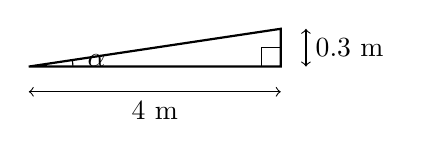
\begin{tikzpicture}[scale=0.8]
    \draw[thick] (0,0) -- (4,0) -- (4,0.6) -- cycle;
    \draw (3.7,0) rectangle (4,0.3);
    \draw[<->] (0,-0.4) -- (4,-0.4) node[midway,below] {4 m};
    \draw[<->] (4.4,0) -- (4.4,0.6) node[midway,right] {0.3 m};
    \draw (0.7,0) arc (0:8.5:0.7) node[right,xshift=2pt] {$\alpha$};
\end{tikzpicture}
\end{center}
}

\subexercicio{Converte a altura para metros.}

\subexercicio{Usa a razão trigonométrica adequada para calcular $\tan(\alpha)$.}

\subexercicio{Calcula o ângulo $\alpha$ (em graus). Usa a calculadora para encontrar $\tan^{-1}$ (arctangente).}

\subexercicio{As normas de acessibilidade recomendam um ângulo máximo de 5°. Esta rampa cumpre a norma? Justifica.}
\FloatBarrier

% Exercício 4: MAT_A12OTIMI_PROB_RAM_002.tex
% Exercise ID: MAT_A12OTIMI_PROB_RAM_002
% Module: Módulo A12 - Otimização | Concept: Problemas Simples de Otimização
% Type: problemas_de_rampas | Difficulty: 2/5
% Tags: trigonometria, rampas, acessibilidade, angulo
% Author: Professor | Date: 2025-11-25

\exercicio{
Um edifício precisa de uma rampa de acesso que suba 50 cm de altura. O projetista quer que a inclinação da rampa seja exatamente de 4° (dentro das normas de acessibilidade).

\begin{center}
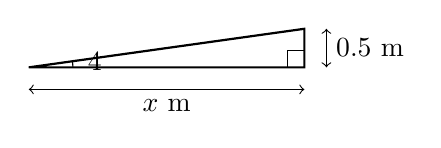
\begin{tikzpicture}[scale=0.7]
    \draw[thick] (0,0) -- (5,0) -- (5,0.7) -- cycle;
    \draw (4.7,0) rectangle (5,0.3);
    \draw[<->] (0,-0.4) -- (5,-0.4) node[midway,below] {$x$ m};
    \draw[<->] (5.4,0) -- (5.4,0.7) node[midway,right] {0.5 m};
    \draw (0.8,0) arc (0:8:0.8) node[right,xshift=2pt] {$4°$};
\end{tikzpicture}
\end{center}
}

\subexercicio{Qual razão trigonométrica relaciona a altura com o comprimento horizontal da rampa?}

\subexercicio{Sabendo que $\tan(4°) \approx 0.07$, calcula o comprimento horizontal $x$ necessário.}

\subexercicio{Qual seria o comprimento total da rampa (hipotenusa)? Usa o Teorema de Pitágoras.}

\subexercicio{Se o espaço disponível é de apenas 6 metros horizontais, a rampa pode ser construída com inclinação de 4°? Justifica.}
\FloatBarrier

% Exercício 5: MAT_A12OTIMI_PROB_TRI_001.tex
% Exercise ID: MAT_A12OTIMI_PROB_TRI_001
% Module: Módulo A12 - Otimização | Concept: Problemas Simples de Otimização
% Type: triangulos_ret_puros | Difficulty: 2/5
% Tags: triangulo_retangulo, vertices, funcao, coordenadas
% Author: Professor | Date: 2025-11-25

\exercicio{
Considera a função $f(x) = x^2$ e o triângulo $[ABC]$ onde:
\begin{itemize}
    \item O vértice $A$ está na origem $(0, 0)$
    \item O vértice $B$ está sobre o gráfico de $f$ no ponto $(2, f(2))$
    \item O vértice $C$ está sobre o eixo $Ox$ tal que $\overline{BC}$ é vertical (perpendicular ao eixo $Ox$)
\end{itemize}
Nota: O triângulo é retângulo em $C$ pois $\overline{BC} \perp \overline{AC}$.
}

\subexercicio{Determina as coordenadas do vértice $B$.}

\subexercicio{Determina as coordenadas do vértice $C$.}

\subexercicio{Calcula a área do triângulo $[ABC]$.}

\subexercicio{Qual seria a área se usássemos $x_B = 3$ em vez de $x_B = 2$?}
\FloatBarrier

% Exercício 6: MAT_A12OTIMI_PROB_TRI_002.tex
% Exercise ID: MAT_A12OTIMI_PROB_TRI_002
% Module: Módulo A12 - Otimização | Concept: Problemas Simples de Otimização
% Type: triangulos_ret_puros | Difficulty: 2/5
% Tags: triangulo_retangulo, vertices, funcao_linear, coordenadas
% Author: Professor | Date: 2025-11-25

\exercicio{
Considera a função $g(x) = 2x + 1$ e um triângulo retângulo $[PQR]$ onde:
\begin{itemize}
    \item O vértice $P$ está sobre o gráfico de $g$ com $x_P = 0$
    \item O vértice $Q$ está sobre o gráfico de $g$ com $x_Q = 3$
    \item O vértice $R$ está sobre o eixo $Ox$ tal que $\overline{PR}$ é vertical
\end{itemize}
}

\subexercicio{Determina as coordenadas de $P$ e $Q$.}

\subexercicio{Determina as coordenadas de $R$.}

\subexercicio{Verifica que o triângulo é retângulo em $R$ calculando o comprimento dos três lados.}

\subexercicio{Calcula a área do triângulo $[PQR]$.}
\FloatBarrier

% Exercício 7: MAT_A12OTIMI_PXX_TRP_001.tex
% Exercise ID: MAT_A12OTIMI_PXX_TRP_001
% Module: Módulo A10 - Otimização | Concept: Problemas Simples de Otimização | Type: Triângulos Retângulos e Funções
% Difficulty: 4/5 (Difícil) | Format: desenvolvimento
% Tags: funcao, triangulo_retangulo, vertices, rampas, triangulos, coordenadas, modelagem, trigonometria, teste, automacao
% Author: Teste Automático | Date: 2025-11-26
% Status: active

\exercicio{Exercício de teste para triangulos_ret_puros}
\FloatBarrier

\end{document}
